\chapter{Introduction}
\noindent
In these times of COVID-19 pandemic, there is a high risk of infections at places where there would be gathering of people like schools/colleges, banks, metro stations, malls, sports stadiums, industries, etc. Till the arrival of vaccines/preventive medicines, the spread must be controlled by safety measures like wearing masks, sanitizing hands and maintaining social distancing. At the entrance of every institution/organization, it would be a daunting exercise to manually test everyone’s body temperature, sanitize everyone’s hands and check for masks, as it is not only time consuming, but also involves the risk of infection to the person doing this job. So, there is a dire need for an automated monitoring system. 
Specifically, in the context of educational institutions, there is a need to integrate the attendance monitoring with appropriate screening. The use of touch-based biometrics needs to be avoided.  Thus, our project aims to build an integrated automated screening and health monitoring system, in addition to recording the attendance by facial recognition.
%\section{Problem Statement}
 %To get accurate and meaningful information using CT and MRI images %with minimum error possible

\section{Motivation}
\begin{enumerate}
	\item SOCIAL IMPACT: We want to do a socially relevant project which would help the community for current needs. \par 
	\item PRODUCT DEVELOPMENT:
We also want to do a project which could be commercialized.
 \par
\end{enumerate}

\section{Objectives}
\begin{enumerate}
	\item 	To monitor the temperature of every person entering the institution  \par 
	\item 	To provide warning messages and inform the concerned authorities/health officials for immediate supportive action (via voice or display), for persons with above normal body temperature.\par 
	\item 	To record the attendance via facial recognition algorithm (via voice or display), for persons having normal temperature.\par
	\item 	To check for proper wearing of the mask (via voice or display). \par 
    \item 	To advice the person to use the hand sanitization system (via voice or display), before proceeding further. \par
\item 	To Catalogue all the details of users to the institution database, on a daily basis.\par
\item 	To calculate the Body Mass Index (weight and height ratio) of a person to gauge their fitness. (exact implementation is still under planning)  \par
\item	To use a contactless heart beat sensor for the measurement of pulse/heartbeat. Even this is used to gauge a person’s fitness. (exact implementation is still under planning) \par
\end{enumerate}

\section{Methodology}
\begin{flushleft}
	\textbf{Steps Invloved in Automated Screening and Health Monitoring System} \begin{enumerate}
		\item BODY TEMPERATURE CHECKING - If the temperature of the user is above normal, our system will immediately inform the concerned person/health official.
 
	\item FACIAL RECOGNITION AND MASK MONITORING -ARM Cortex processor which is capable of handling image processing and deep learning algorithms is used.Our health monitoring and screening system has a camera attached to it. With the help of this camera and using the concepts of image processing and deep learning, the attendance of the person is recorded based on facial recognition.Using the same concepts, the system also checks whether the person is wearing the mask or not.

	\item INDICATING THE PARAMETERS - LCD display, LEDs and buzzer are used to indicate parameters of the user like temperature, time of entry, mask detection and name of the person. 

	\item AUTOMATED HAND SANITIZER - Our system also includes, an automated hand sanitizer unit. It has an IR sensor, a DC water pump, transistor and resistors. It is a touch free hand sanitizer dispensing system. This system is independent which works only with DC power supply and not controlled by the ARM processer (as depicted in the block diagram below).
.\end{enumerate}  \end{flushleft}

\section{Applications and Future Scope}
\begin{enumerate}
	\item 	This integrated system can be used at the entrance of educational institutions, metro stations, industries, banks, malls, etc. to screen every individual for his body temperature, mask wearing and hand sanitization. \par 
	\item The system helps in cataloguing the details of users/entrants to an appropriate database \par
 \item 	The system may be made to provide health tips to needy individuals during the leisure time of the system \par
 \item 	The system could be modified to integrate ‘Aarogyasetu App’ as ‘health assistant \par
\end{enumerate}

\begin{figure}[H]
	\centering
	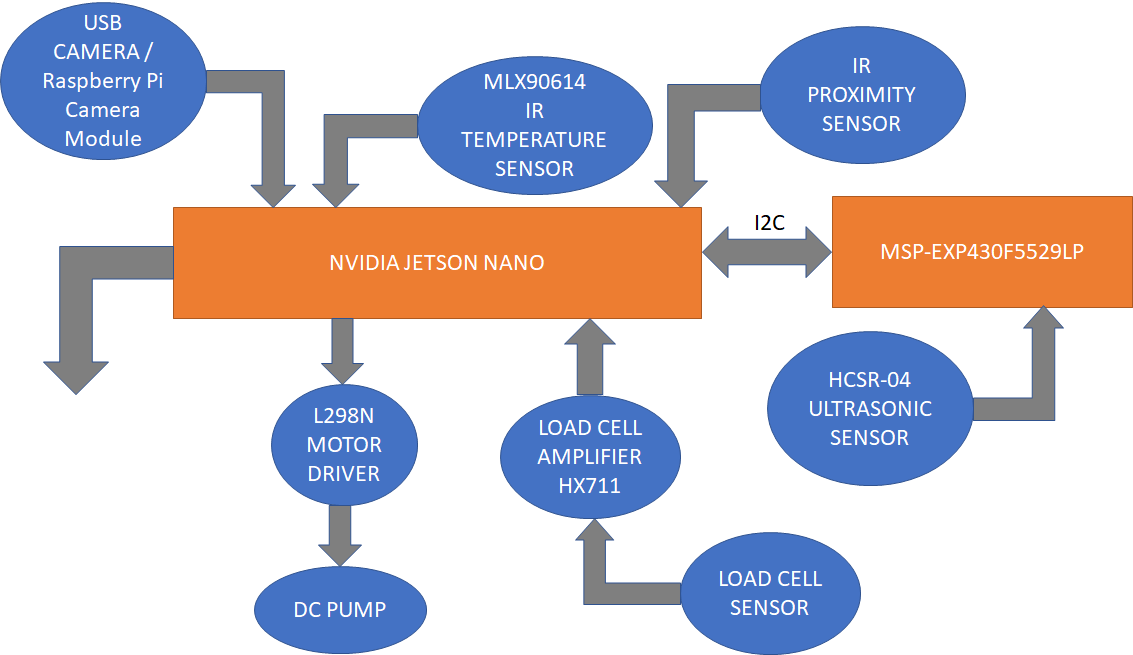
\includegraphics[width=0.7\linewidth]{images/updated bd}
	\caption{Proposed System Block Diagram}
	\label{fig:updated bd}
\end{figure}


		
%\end{flushleft}
